%%%%%%%%%%%%%%%%%%%%%%%%%%%%%%%%%%%%%%%%%
% Journal Article
% LaTeX Template
% Version 2.0 (February 7, 2023)
%
% This template originates from:
% https://www.LaTeXTemplates.com
%
% Author:
% Vel (vel@latextemplates.com)
%
% License:
% CC BY-NC-SA 4.0 (https://creativecommons.org/licenses/by-nc-sa/4.0/)
%
% NOTE: The bibliography needs to be compiled using the biber engine.
%
%%%%%%%%%%%%%%%%%%%%%%%%%%%%%%%%%%%%%%%%%

%----------------------------------------------------------------------------------------
%	PACKAGES AND OTHER DOCUMENT CONFIGURATIONS
%----------------------------------------------------------------------------------------

\documentclass[
	a4paper, % Paper size, use either a4paper or letterpaper
	10pt, % Default font size, can also use 11pt or 12pt, although this is not recommended
	unnumberedsections, % Comment to enable section numbering
	twoside, % Two side traditional mode where headers and footers change between odd and even pages, comment this option to make them fixed
]{LTJournalArticle}

\addbibresource{sample.bib} % BibLaTeX bibliography file

\runninghead{Food recognition and leftover estimation} % A shortened article title to appear in the running head, leave this command empty for no running head

\footertext{\textit{Computer Vision course} (2022-2023)} % Text to appear in the footer, leave this command empty for no footer text

\setcounter{page}{1} % The page number of the first page, set this to a higher number if the article is to be part of an issue or larger work

%----------------------------------------------------------------------------------------
%	CODE SECTION
%----------------------------------------------------------------------------------------

\usepackage{listings}
\usepackage{color}

\definecolor{codegreen}{rgb}{0,0.6,0}
\definecolor{codegray}{rgb}{0.5,0.5,0.5}
\definecolor{codepurple}{rgb}{0.58,0,0.82}
\definecolor{backcolour}{rgb}{0.95,0.95,0.92}

\lstdefinestyle{mystyle}{
    backgroundcolor=\color{backcolour},
    commentstyle=\color{codegreen},
    keywordstyle=\color{magenta},
    numberstyle=\tiny\color{codegray},
    stringstyle=\color{codepurple},
    basicstyle=\ttfamily\footnotesize,
    breakatwhitespace=false,
    breaklines=true,
    captionpos=b,
    keepspaces=true,
    numbers=false,
    numbersep=5pt,
    showspaces=false,
    showstringspaces=false,
    showtabs=false,
    tabsize=2,
    language=C++
}

%----------------------------------------------------------------------------------------
%	TITLE SECTION
%----------------------------------------------------------------------------------------

\title{Food Recognition and Leftover Estimation} % Article title, use manual lines breaks (\\) to beautify the layout

% Authors are listed in a comma-separated list with superscript numbers indicating affiliations
% \thanks{} is used for any text that should be placed in a footnote on the first page, such as the corresponding author's email, journal acceptance dates, a copyright/license notice, keywords, etc
\author{Pietrobon Andrea,}

% Affiliations are output in the \date{} command
\date{Department of Engineering Information, University of Padua}

% Full-width abstract
\renewcommand{\maketitlehookd}{%
	\begin{abstract}
		\noindent In this research, I present my revision of the previous group project, enhancing the capabilities and improving various aspects. Let's start with a premise. In the design phase, I chose to avoid using a neural network for food identification because the entire course was conducted in the C++ language and primarily emphasized the use of various image processing techniques unrelated to neural networks. Therefore, even though I was aware that using a neural network could have significantly improved the results, I opted to continue using openCV and the techniques learned in class. The current project is primarily divided into four phases: food localization, aimed at identifying the precise location of various foods in the image to enclose them within a bounding box; segmentation, which aims to remove unnecessary parts of the image from the bounding box and identify only the pixels containing food; classification, with the objective of identifying which foods are present in the image and their respective quantities; and finally, the results estimation phase, which measures the accuracy of the three aspects mentioned earlier. \end{abstract}}

%----------------------------------------------------------------------------------------

\begin{document}

\maketitle % Output the title section

%----------------------------------------------------------------------------------------
%	ARTICLE CONTENTS
%----------------------------------------------------------------------------------------
\textbf{NOTE: As indicated by the professor, the trays used represent the entire available world and no limitations have been imposed on temporal and spatial complexity.}

\section{Introduction}
The code structure for identifying food and estimating leftovers is quite simple.
As anticipated, it is mainly divided into 4 macro sections.
These macro sections are:
\begin{enumerate}
	\item Food Localization
	\item Food Segmentation
	\item Food Classification
	\item Results and Performance metrics
\end{enumerate}

In this introductory part, we will focus on the main structure of the code, leaving out the macro areas indicated in the specific sections. The fundamental idea is to load the images of each tray one at a time and commence with Food Localization, which will be responsible for cleaning the image from objects or parts that are irrelevant or do not contain food, in order to more precisely identify the boxes for each course and/or food.

Once the bounding boxes in the image have been detected, they are passed on to the next section, which will take care of refining and perfecting them through food segmentation, preparing them for classification. This operation also has a "side effect" that further improves the bounding boxes found in the previous section.

At this point, a vector containing each dish present in the image will be returned. For instance, in Figure \ref{fig:tray4.1}, there are two different courses with three different foods (pasta with tomato sauce, fish, and potatoes), a side dish (salad), and bread. Consequently, the vector will contain five segmented foods.

\begin{figure}[t]
    \centering
    \includegraphics[width=0.47\textwidth]{Images/food_image_tray4.1.jpg}
    \caption{First image of the tray 4}
    \label{fig:tray4.1}
\end{figure}

After completing the previous steps, the vector containing the outlines of the foods found in the image is passed to the classification section. This part of the code relies on the colors, shapes, and brightness of the image to identify the types of food. \textbf{This procedure was chosen instead of a more efficient and high-performing method like SIFT or ORB. The reason for this choice is due to the very limited size of the dataset and the lack of usable features, which would have led to further reduction of the dataset by using some images as features. I considered the option of using images from the internet to identify various foods, but due to uncertainty about the appropriateness of using external images, I opted for the method described above. Nevertheless, I have initiated the implementation of the SIFT method (to be completed) to have both methodologies available. In any case, in a real-world scenario, the use of SIFT is significantly more effective, as manually writing code to identify foods would be complex and require substantial time and resources.}

In figure \ref{fig:Vector} there is a graphical representation of a simplified vector to help imagine what is contained in the main vector.

\begin{figure}[t]
    \centering
    \includegraphics[width=0.25\textwidth]{Images/Vector.png}
    \caption{Main Vector with the results}
    \label{fig:Vector}
\end{figure}

At the same time, at each iteration in each image, the bounding boxes will be drawn for each food with the relative label. Which will be saved and merged with the other tray images at the end to show the final result.

The \ref{tab:percentage} table shows an example of the results for the Tray 1. \\

\begin{table} % Single column table
	\caption{Example of the output information for the first tray.}
	\centering
	\begin{tabular}{l l r}
		\toprule
		Images of tray X & Food present & \% food left \\
		\midrule
        Image 1 & Pasta with pesto & 100\% \\
                      & Grilled pork cutlet & 100\% \\
                      & Beans & 100\% \\
                      & Bread & 100\% \\
        \\
        Image 2 & Pasta with pesto & 60\% \\
                      & Grilled pork cutlet & 80\% \\
                      & Beans & 95\% \\
                      & Bread & 80\% \\
        \\
        Image 3 & Pasta with pesto & 20\% \\
                      & Grilled pork cutlet & 50\% \\
                      & Beans & 75\% \\
                      & Bread & 60\% \\
        \\
        Image 4 & Pasta with pesto & 0\% \\
                      & Grilled pork cutlet & 0\% \\
                      & Beans & 60\% \\
                      & Bread & 30\% \\
		\bottomrule
	\end{tabular}
	\label{tab:percentage}
\end{table}


%To independently test the code, simply follow these steps:

To independently test the code, simply download the folder containing the code and the dataset. Then, through the terminal, you need to run the following commands (replace "FOLDER-NAME" with the name of the folder where all the files are located):
More information can be found at the following \href{https://github.com/Piero24/Food-recognition-and-leftover-estimation}{link}.


\begin{lstlisting}[breaklines=true]
make

./FOLDER-NAME ./Food-recognition-and-leftover-estimation/dataset
\end{lstlisting}

%------------------------------------------------

\section{Food localization}

To locate the food, I have chosen to operate using different methodologies, which will then be combined to give a better and more accurate result. In fact, both of the chosen approaches led to some errors when used individually in food detection, preventing the identification of some dishes in some trays. By combining these operations together, I was, therefore, able to improve the general selection of dishes.

Initially, three different methodologies had to be used, but subsequently, given the good results, I opted for the use of only two different methods. The first, after an initial preprocessing on the image, finds the food based on the pixels left on the image, while the second one takes advantage of the circular shape of the dishes to find the main courses.

As introduced earlier, this approach of using different methodologies allows compensating for each other's shortcomings. In fact, if the dishes had been square or of shapes other than circular, it would have been impossible to locate them correctly with only one of the two chosen methods, and therefore the operations would not have been successful. Or again, it would not have been possible to locate the bread correctly in all images since it is not positioned on any circular surface.

\subsection{Preprocessing}
As the first operation after importing the original tray images we apply a preprocessing on them.
This operation is made up of various processes made to the image which allow you to remove unnecessary parts and therefore which are not part of the food such as for example: Plates, trays and cutlery.
To remove them, some operations were used such as: Canny edge detector, erosion and dilatation. In addition, operations were used to remove specific colors that were on all or some of the images and were not part of the food.

\begin{figure}
    \centering
    \subfigure{\includegraphics[width=0.4\textwidth]{Images/food_image_tray1.1.jpg}} 
    \subfigure{\includegraphics[width=0.4\textwidth]{Images/ImagePreprocessed_tray_1.1.jpg}} 
    \caption{Image 1 of the first tray (a) Original image (b) Processed image}
    \label{fig:prepcompare}
\end{figure}

As can be seen from the images in figure \ref{fig:prepcompare} these processes have helped a lot in the detection phase by completely or almost eliminating the excess components that were not part of the food. However, some parts of the food have been eroded by these operations, such as the central part of the bread or some sections of the dough. This is due to the elimination from the image of some specific portions of color which were also present in the foods. However, since they are not essential for the localization operation, this compromise has been reached.

\subsection{Rectangular Bounding Boxes}
I started by creating the recSegmentation function (figure \lstlistingname~\ref{lst:codice}) which uses SelectiveSearchSegmentation to find the various rectangles in the image, based on 2 main elements: Color and Texture.


\lstset{style=mystyle}
\begin{lstlisting}[caption=recSegmentation, label=lst:codice]
std::vector<cv::Rect> recSegmentation(cv::Mat img, std::string quality) {

    cv::Ptr<cv::ximgproc::segmentation::SelectiveSearchSegmentation> ss = cv::ximgproc::segmentation::createSelectiveSearchSegmentation();

    cv::Ptr<cv::ximgproc::segmentation::SelectiveSearchSegmentationStrategy
    Color> colorStrategy = cv::ximgproc::segmentation::createSelectiveSearch
    SegmentationStrategyColor();
    
    cv::Ptr<cv::ximgproc::segmentation::SelectiveSearchSegmentationStrategy
    Texture> textureStrategy = cv::ximgproc::segmentation::createSelective
    SearchSegmentationStrategyTexture();
    
    cv::Ptr<cv::ximgproc::segmentation::SelectiveSearchSegmentationStrategy
    Multiple> multipleStrategy = cv::ximgproc::segmentation::createSelective
    SearchSegmentationStrategyMultiple(colorStrategy, textureStrategy);

    ss -> addStrategy(multipleStrategy);
    ss -> setBaseImage(img);

    if (quality == "f") {
        ss -> switchToSelectiveSearchFast();

    } else {
        ss -> switchToSelectiveSearchQuality();
    }

    std::vector<cv::Rect> rects;
    ss -> process(rects);

    return rects;
}
\end{lstlisting}

 This allowed me to quickly find many bounding boxes within the image. Obviously not only and exclusively the requested boxes found, but most of them were useless to achieve our goal. For this reason, I skimmed the boxes found. I therefore developed the removeInnerRectangles function (figure \lstlistingname~\ref{lst:code2}) which removes the rectangles that overlap or are contained in other rectangles already identified.
  
\lstset{style=mystyle}
\begin{lstlisting}[caption=removeInnerRectangles, label=lst:codice2]
std::vector<cv::Rect> removeInnerRectangles(const std::vector<cv::Rect>& rectangles) {
    std::vector<cv::Rect> result;

    for (const cv::Rect& rect : rectangles) {
        bool isInner = false;

        for (const cv::Rect& existingRect : result) {
            if (isOverlap(rect, existingRect)) {
                isInner = true;
                break;
            }
        }

        if (!isInner) {
            result.push_back(rect);
        }
    }

    return result;
}
\end{lstlisting}

In doing so I removed most of the bounding boxes that weren't needed, that were duplicates or that didn't find the various foods correctly. As a last step, however, I removed the remaining incorrect boxes by exploiting the pixel density. Some of the boxes in fact found isolated pixels which were not part of any range. For this reason I calculated the number of non-black pixels inside each remaining box and kept only the boxes with a density higher than a certain threshold value. This allowed me to keep only the most accurate boxes by permanently deleting anything that wasn't relevant.

\begin{figure}[t]
    \centering
    \includegraphics[width=0.47\textwidth]{Images/RecBoxes_tray1.1.jpg}
    \caption{Food localized with recSegmentation}
    \label{fig:RecBoxes11}
\end{figure}

\begin{figure}[t]
    \centering
    \includegraphics[width=0.47\textwidth]{Images/RecBoxes_tray4.4.jpg}
    \caption{Problem with some leftovers}
    \label{fig:RecBoxes_tray4.4}
\end{figure}

The image in figure~\ref{fig:RecBoxes11} shows the final result obtained in the image with the use of the function specified here only.

However, as can be seen in figure~\ref{fig:RecBoxes_tray4.4} some portions of food (the potatoes at the top left) due to the processing done to the image in the preprocessing function are not detected. And this main problem was what prompted me to use 2 different methods to then merge the results obtained.

\subsection{Circular Bounding Boxes}
This second detection function is based on HoughCircles, which allowed me to find the dishes in the image. Since the photos were taken at different angles and at different distances from the various trays, the size of the dishes varied considerably. I solved this problem by first working on the larger circles and then on the smaller diameter circles so as to be more precise in recognizing the dish.

Starting from the circles with bigger dimension or developed the biggerCirclesPreprocessing function, which applied some preprocessing to the image. Specifically I went to transform the image in grayscale and then with the use of Canny edge detector and a Gaussian Blur I created the image on which I was going to work.

The next step was to use HoughCircles to find the largest circles. In this way, the output vector \texttt{std::vector<cv::Vec3f> biggerCircles} contains all the circles found. Unfortunately also in this case as in the recSegmentation function, the vector contained many overlapping circles and some were completely wrong. To solve this problem and therefore have a single circle for each plate I noticed that most of the circles had more or less the same center. So I thought we'd use this to our advantage.

To keep only one circle of the right size for each plate I have therefore chosen to use an "artisanal" clustering technique. The basic idea is to compare one by one the distance of the centers of the various circles. If the distance is less than a pre-established threshold value, the given circle is added to the cluster and calculate its weighted average which will act as a centroid. If the distance between the centers of the circles and the centroid is greater than the threshold value I create a new cluster and add the circle to it. By iterating this procedure for all the circles, I will have a vector containing the clusters with the various circles which I will then sort according to the number of circles for each cluster. Indeed, the clusters with the highest number of circles are those corresponding to the dishes. While clusters with a low number of circles are only HoughCircles errors and can be discarded. In figure~\ref{fig:CircBoxes_nocluster_tray6.1} there is a representation of the circles found in an image with HoughCircles before applying the previously indicated approach (The code is not shown below for the only reason that it would take up too much space. You can see the function in the file: circularBoundingBoxes.cpp). 

\begin{figure}[t]
    \centering
    \includegraphics[width=0.47\textwidth]{Images/CircBoxes_nocluster_tray6.1.jpg}
    \caption{Circles found with HoughCircles}
    \label{fig:CircBoxes_nocluster_tray6.1}
\end{figure}

At this point, the clusters contained varying amounts of circles and only one circle had to be kept for each plate discarding all the extra and incorrect circles. So I counted the number of circles and kept only the clusters with a number of circles above a certain threshold value.

Concluded with the larger circles I repeated the process with the smaller size image circles slightly changing the preprocessing method and adding a variation to the clustering methodology. In fact, in the phase of checking the various circles present in each cluster, it is verified that the smallest circle was not contained in one of the larger circles. If so, the circle is discarded, otherwise being external it is considered as a plate. Figure~\ref{fig:CircBoxes_tray6.1} shows the final result of the clustering technique.

\begin{figure}[t]
    \centering
    \includegraphics[width=0.47\textwidth]{Images/CircBoxes_tray6.1.jpg}
    \caption{Circles left after using kmenasCircle}
    \label{fig:CircBoxes_tray6.1}
\end{figure}

The function that implements this clustering technique is called kmenasCircle. Because the original idea was to use kmenas as a clustering methodology but as we know one of the main problems of this technique is the fact that the number of clusters k has to be provided in advance. However, this prevented the implementation of this approach since the dataset had a variable amount of dishes with each image.
(The name has remained unchanged solely for the purpose of remembering from which clustering technique the initial inspiration for implementing this technique was taken).

\begin{figure}[t]
    \centering
    \includegraphics[width=0.47\textwidth]{Images/CircBoxes_tray5.3.jpg}
    \caption{Problem on detecting bread with HoughCircles}
    \label{fig:CircBoxes_tray5.3}
\end{figure}

\begin{figure}[t]
    \centering
    \includegraphics[width=0.47\textwidth]{Images/CircBoxes_tray4.2.jpg}
    \caption{Problem on detecting some circles}
    \label{fig:CircBoxes_tray4.2}
\end{figure}

However, as anticipated at the beginning of the chapter, some problems arose in this case as well. In fact some foods (such as bread) are not present inside the plate as it is possible to see in the figure~\ref{fig:CircBoxes_tray5.3} this therefore prevented using this approach to detect it. Another problem was found in the figure~\ref{fig:CircBoxes_tray4.2} where the plate was not completely present within the image and this prevented a correct localization of the food which, however, happened correctly with the use of recSegmentation.

\subsection{Merging Method}
After preparing the vectors containing the rectangular bounding boxes obtained from "findRectangularBoundingBoxes" and the circular ones obtained from "findCircularBoundingBoxes," it was necessary to merge the two vectors. To do this, I developed the "subjectIsolator" function with three main objectives. The first is to merge the overlapping elements between the two vectors; for example, if I have a plate of pasta that has been detected by both functions as shown in figure~\ref{fig:merginbox_tray1.1}, I can overlay the two masks and keep only the portion of the image that interests me (as can be seen in figures~\ref{fig:mask}, where there are masks for the rectangle only, the circle only, the intersections, and the final one). The second function is to assist when there are multiple rectangular bounding boxes on the same circular bounding box. In case of errors, it helps recreate a single bounding box that contains both rectangles. The third and final function is to retain the parts detected by only one of the two methods, such as bread, for example. This has significantly improved another part of the work. In fact, thanks to this function, I was able to effectively eliminate any false positives (portions of images detected as food) and delineate the main part of the work, which is to segment the food by tracing its contours with greater precision. As will be explained in the following sections, the next objectives will be to segment the food and classify it into various categories, and finally, calculate the amount of wasted food for each tray.\\

\begin{figure}[t]
    \centering
    \includegraphics[width=0.47\textwidth]{Images/merginbox_tray1.1.jpg}
    \caption{Overlap of the 2 methods}
    \label{fig:merginbox_tray1.1}
\end{figure}

\begin{figure}[t]
\centering
    \subfigure{\includegraphics[width=0.2\textwidth]{Images/Mask2.jpg}} 
    \subfigure{\includegraphics[width=0.2\textwidth]{Images/Mask3.jpg}}
    \subfigure{\includegraphics[width=0.2\textwidth]{Images/Mask1.png}} 
    \subfigure{\includegraphics[width=0.2\textwidth]{Images/Mask4.png}} 
    \caption{Obtained masks, intersection mask and final mask}
    \label{fig:mask}
\end{figure}

Below are some of the final results obtained from this merge. To demonstrate its effectiveness in overlapping the bounding boxes are of rectangular and circular shapes in order to show their correct overlapping. However the code as shown below will transform the circular bounding boxes into rectangular shape.

\begin{figure}[t]
    \centering
    \subfigure{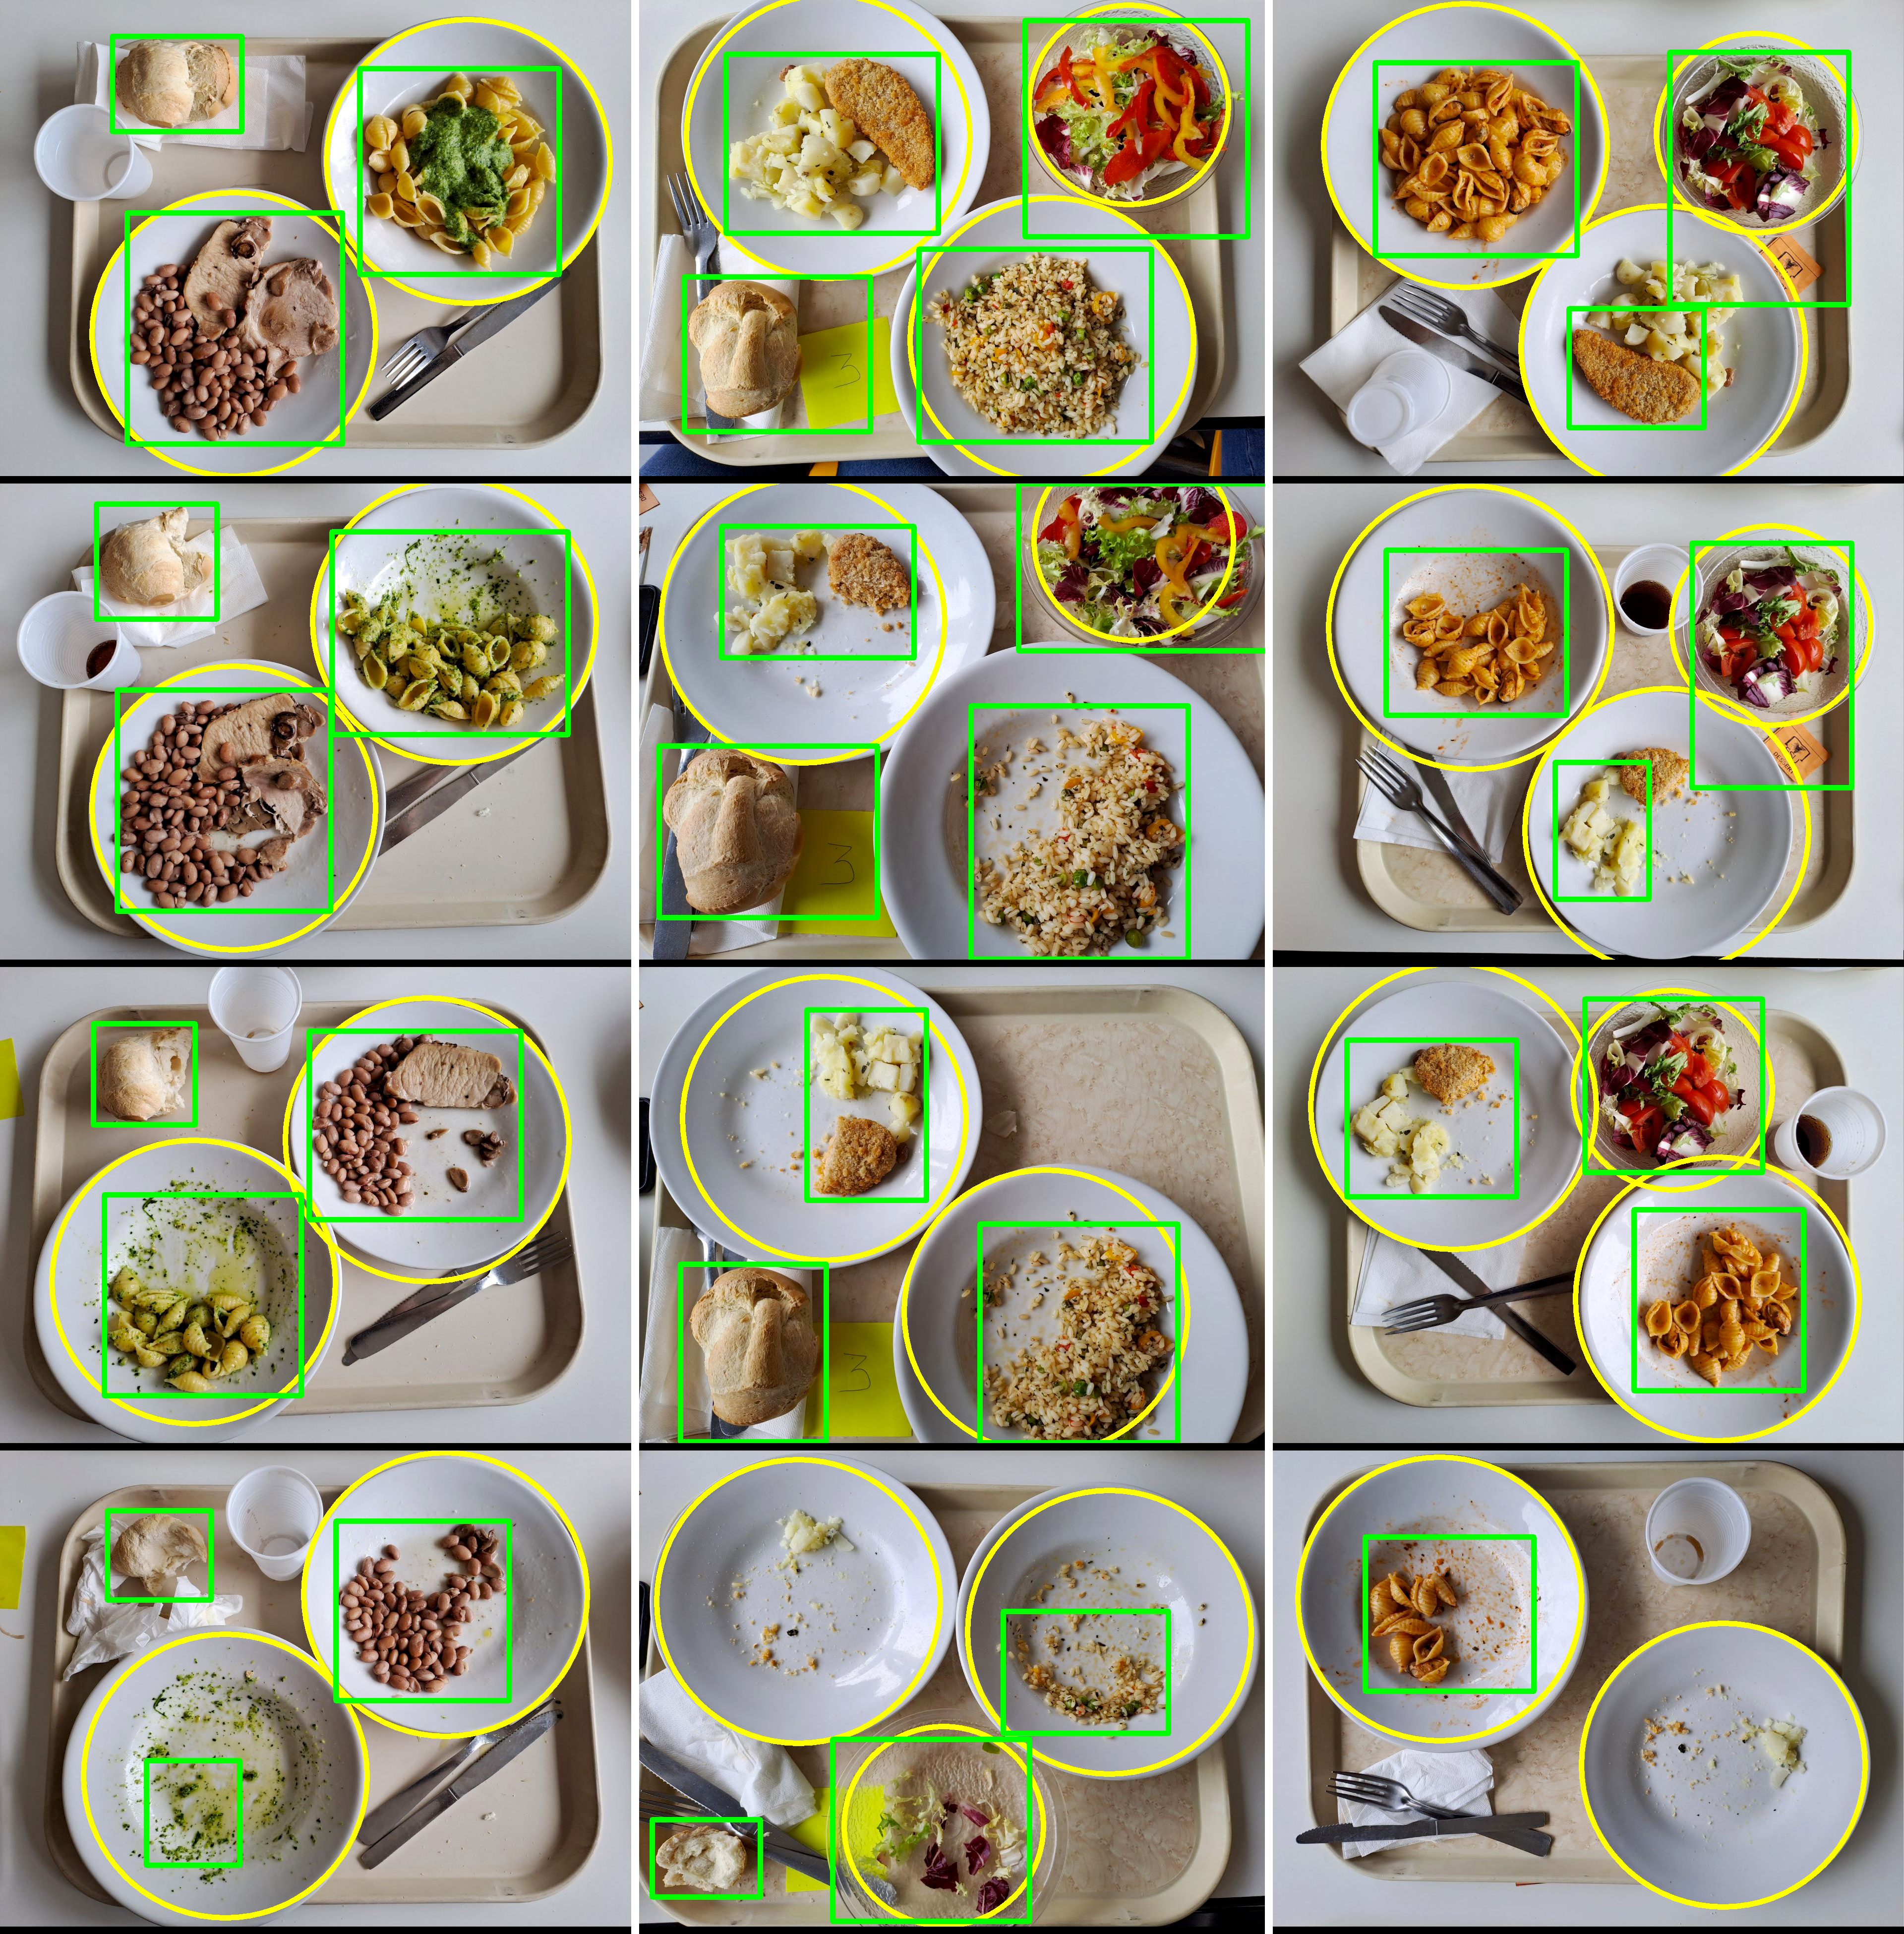
\includegraphics[width=0.47\textwidth]{Images/FinalMergeBBox.png}} 
    \caption{Final results for 3 different trays}
    \label{fig:FinalMergeBBox}
\end{figure}

\section{Food Segmentation}
\subsection{Food bounding boxes}
Once I obtained the various bounding boxes for each dish, I decided to take the original image, obscure everything outside of the bounding box, and retain everything inside. This decision was made due to the erosions and the Canny filter, as these processes could result in the loss of information about certain food items. By preserving only the information contained within the specific bounding box of the dish in question and eliminating the rest, it becomes easier to clean the images of unnecessary information and retain only the food pixels.
After applying a median filter to the image to reduce gradients, we reapplied the Canny algorithm, followed by an erosion process. During this phase, I recognized that pixels with very similar color channels were not relevant to our problem. In particular, channel values with a difference of less than 45 were considered noise and thus removed from the mask.
However, despite these removal operations, food detection was still not optimal. To address this situation, I performed an opening operation by combining erosion and dilation on the mask, using a 9x9 square kernel. (figure \ref{test_2}).\\

\begin{figure}
    \centering
    {\includegraphics[width=0.4\textwidth]{Images/Test_3.png}} 
    \caption{Example on the first image of the first tray}
    \label{test_2}
\end{figure}

After refining the various bounding boxes, I once again stored the resulting contours in a vector, which proved to be more precise than the previous ones. At this point, I tackled one of the main challenges of this project: the need to separate main dishes from contours. As you can see in Figure \ref{fig:tray4.1}, a dish can contain different foods, and I had to find a way to separate the foods only on plates where they were present, without altering the plates with only one type of food (such as pasta with pesto, which exhibits two distinct colors in the first image, which could erroneously appear as different foods).

To address this challenge, I chose to use the K-Means algorithm to identify the predominant colors in the image. Thanks to this clustering algorithm, I quickly isolated the main colors present in the image. This allowed me to exclude many dishes with a predominant color that differed. For example, the fish cutlet and potatoes had distinct predominant colors (light brown and a yellow tending towards white, respectively), which K-Means readily identified, guiding me on which plates to focus on for separating various food types.

Once the target plates were identified, I performed various operations such as Canny edge detection, erosions, dilations, and removal of different colors for each type of plate. Additionally, for some dishes, I calculated the areas of the various contours in the image and, based on a threshold slightly below the average area, retained only the main food portions, eliminating small areas considered as noise. Through the dilation operation, I restored food portions, giving them a more defined and precise outline. An initial result of this process is visible in Figure \ref{fig:Seafood}, where this procedure is applied to Tray 8, Image 1, which contained seafood salad, beans, and potatoes..\\

\begin{figure}[t]
\centering
    \subfigure{\includegraphics[width=0.2\textwidth]{Images/SeafoodTot.png}} 
    \subfigure{\includegraphics[width=0.2\textwidth]{Images/OnlySeafood.png}}
    \subfigure{\includegraphics[width=0.2\textwidth]{Images/OnlyBeans.png}} 
    \subfigure{\includegraphics[width=0.2\textwidth]{Images/OnlyPotatoes.png}} 
    \caption{Separation of seafood salad plate, beans and potatoes}
    \label{fig:Seafood}
\end{figure}

At this stage, the segmentation of various foods is complete, and all individual food items are placed in a contour vector to be passed to the next function, the "foodClassifier." As explained later, the "foodClassifier" function will handle the classification of the various food items.

\section{Food Classification}
\subsection{The Sift algorithm}
For this final part, as previously mentioned, I initially considered using an algorithm like SIFT or ORB to perform food matching based on features. However, this methodology, when applied to this specific case, comes with the following problems:

\begin{enumerate}
	\item Using an external database with features
	\item A possible reduction of the already very small dataset (in case it is not possible to use external images)
\end{enumerate}

In the ideal scenario for a real-world application, not limited to the current dataset \textbf{(which is considered in this project as the entire realm of possibilities)}, the use of SIFT or ORB would be crucial to significantly enhance the capabilities of our program. These approaches would greatly expedite the classification phase, simultaneously increasing accuracy and substantially reducing false positives.

The method I ultimately opted for is quite similar to the one previously employed to separate foods within the same dish. This is made feasible by the fact that the dataset encompasses a limited number of food items. This allows us to individually operate on each food item for accurate classification. If the dataset were more extensive, achieving classification with this procedure would be extremely challenging in terms of scalability, leaving no alternative but to resort to methods like SIFT.

The "foodClassifier" function for classification employs k-means to identify the primary colors of the various food items. The image containing only the food within the contour and the centroid vector are subsequently used by the "foodIdentifier" function. The latter identifies the food type based on color and luminance, employing techniques like erosion, dilation, and Gaussian Blur, as mentioned earlier. Once the food type within the input contour is identified, the classification is returned to the "foodClassifier" function. This function then creates an object of type "Food," containing the food's name, its contour, and additional information, such as the specific color for that food to be used in the bounding box, etc.

Upon completion of these procedures, we will have traversed the three primary phases of our program, resulting in a vector containing objects of type "Food." This vector will be used to create bounding boxes in the image and calculate food surplus. Below, you will find some of the results obtained from various trays. To view all the results obtained, please visit the following \href{https://github.com/Piero24/Food-recognition-and-leftover-estimation}{link}.

\begin{figure}[t]
    \centering
    \subfigure{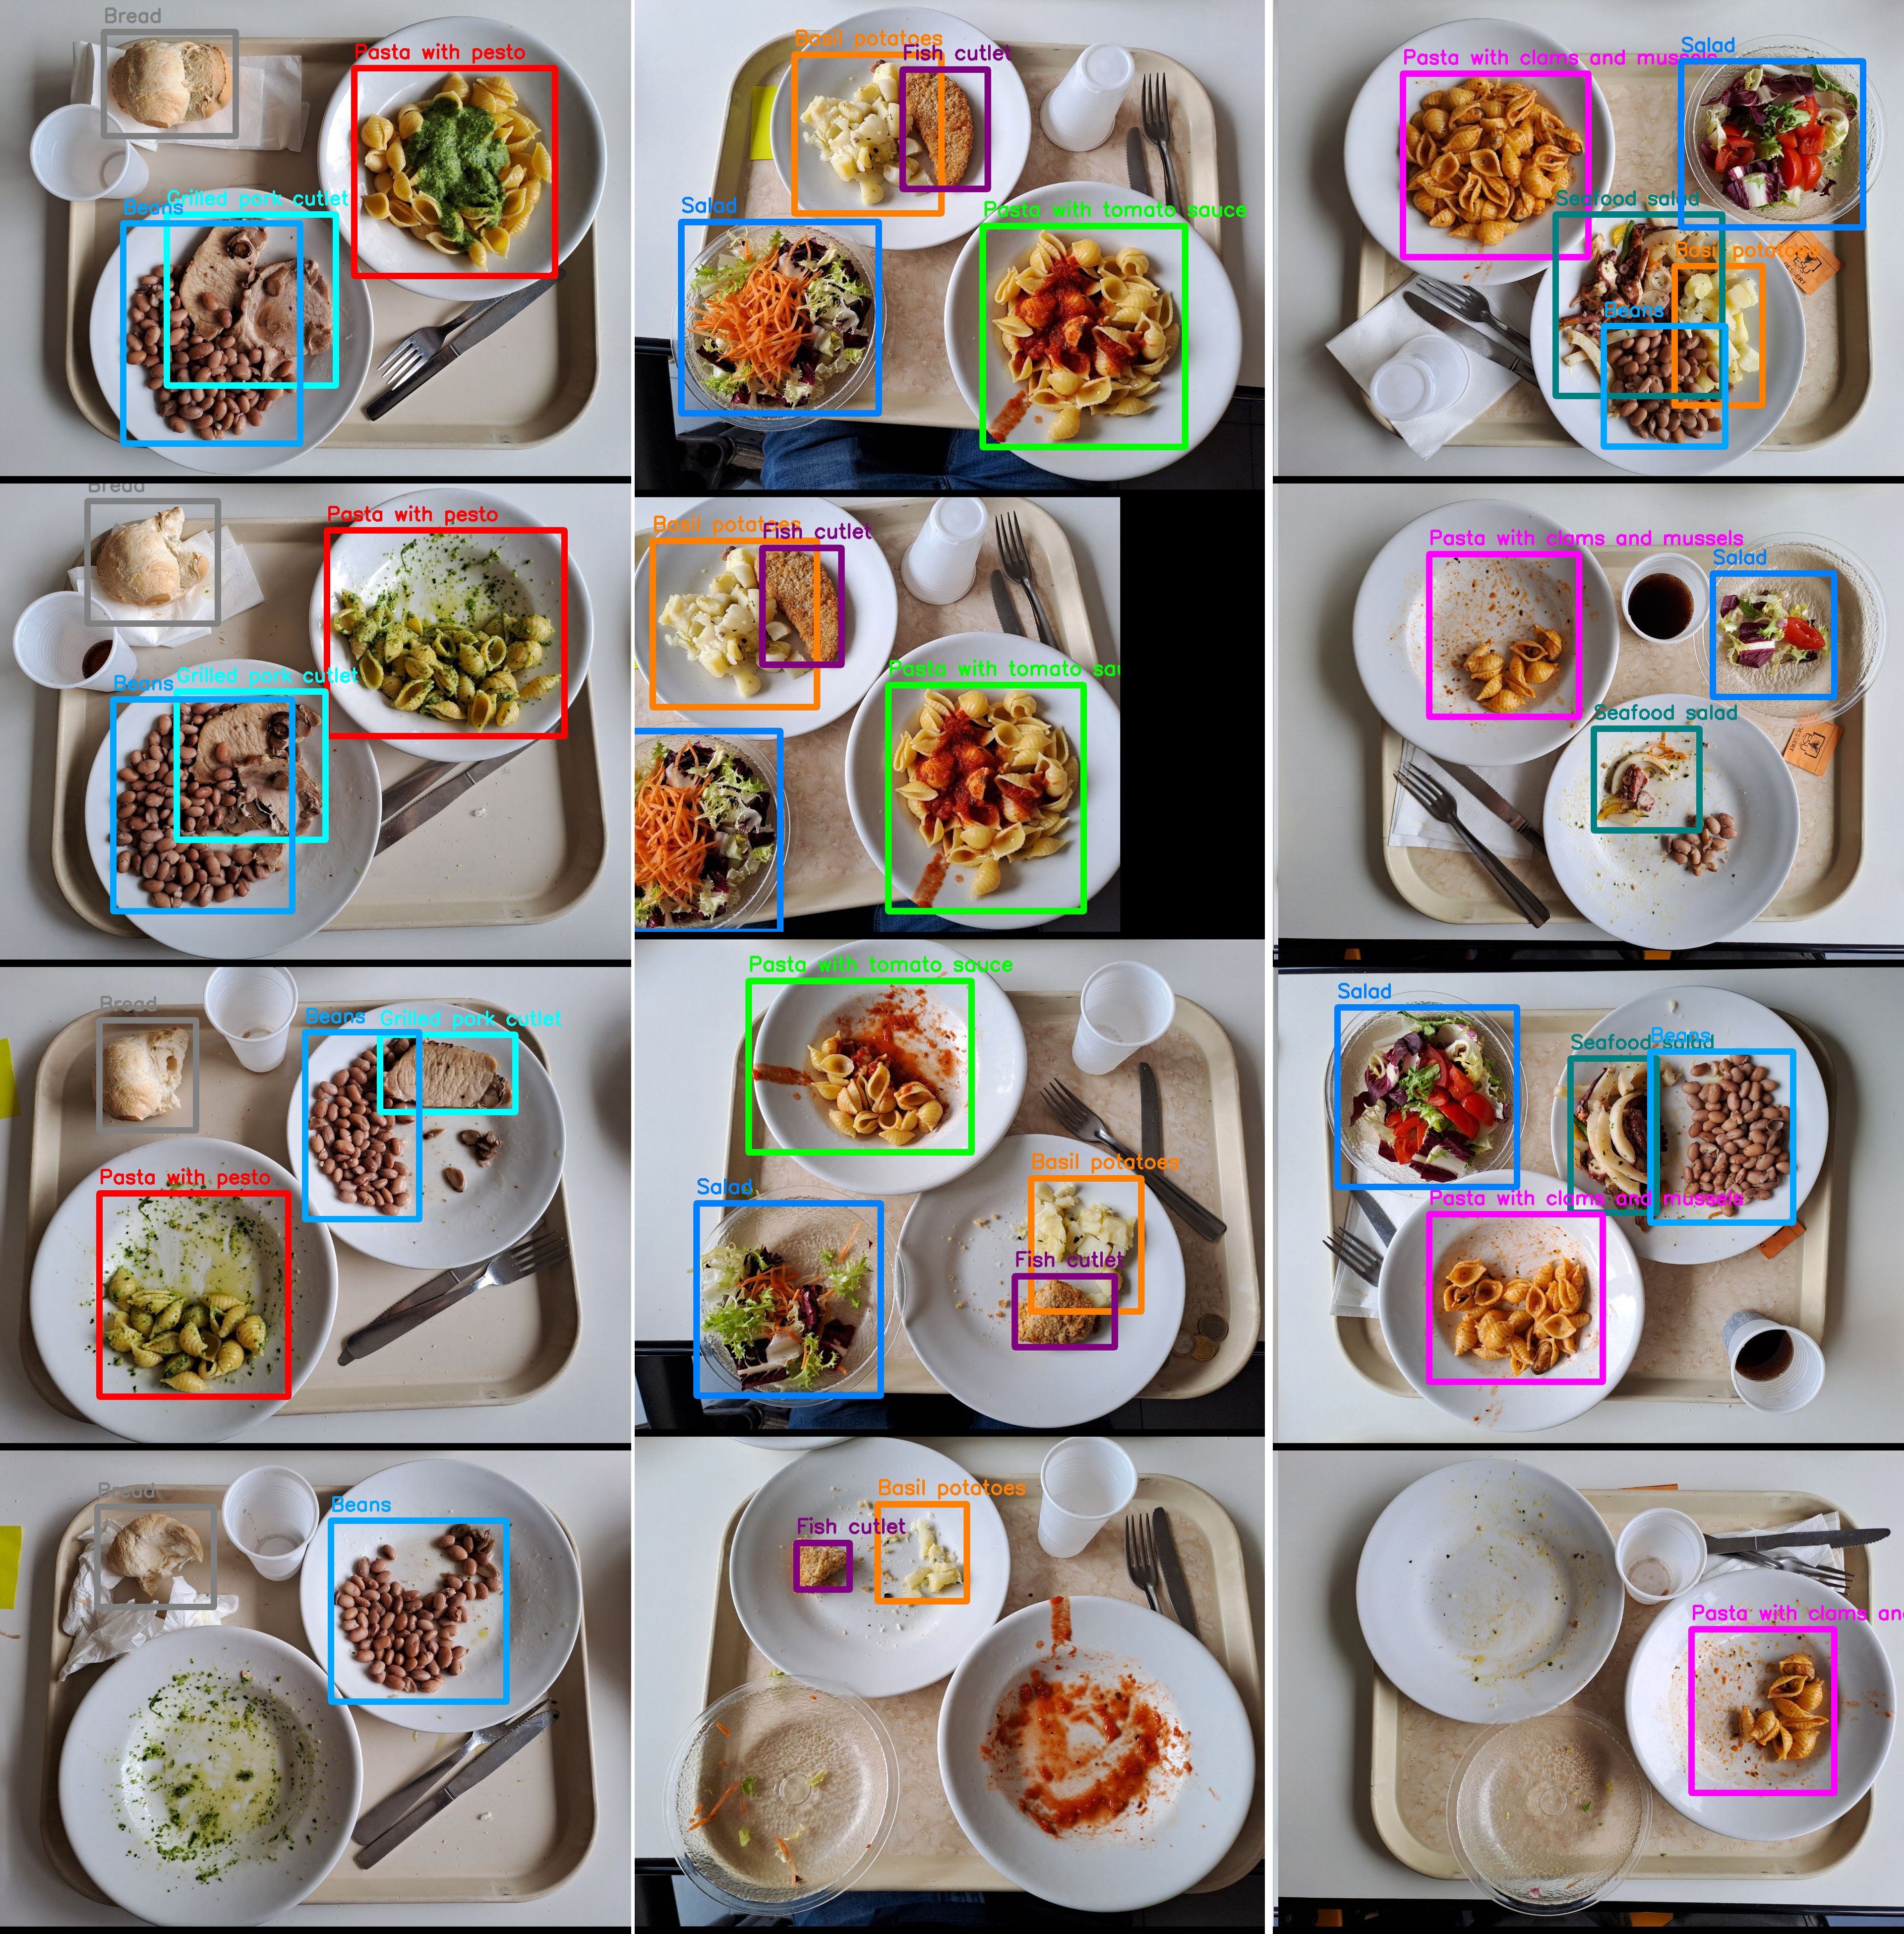
\includegraphics[width=0.47\textwidth]{Images/final3trays.png}} 
    \caption{Final results for 3 different trays (1, 2 and 8)}
    \label{fig:Final3trays}
\end{figure}

\textbf{NOTE: A modified version of this program using SIFT is currently under construction to evaluate the differences between the two methods. It will be added later with the option for the user to choose which method to use.}

%------------------------------------------------















\section{Results}
Due to the lack of the part of the code dedicated to the classification of foods, we could not proceed further.
In fact, this prevented us from assigning the correct label to each bounding box and therefore from categorizing the various foods according to the type of belonging and in turn from carrying out the required tests, namely:
\begin{enumerate}
	\item The mean Average Precision (mAP)
	\item The  mean  Intersection  over  Union  (mIoU)
\end{enumerate}

Furthermore, it was not possible to produce an estimate for all the leftover foods as without a correct classification it is not possible to understand which dishes correspond to the leftovers left in the various dishes.

\subsection{For food leftover estimation}
The method leftFood take all the names from the imageNames and sort them based on alphabetical order according to an index array as support . In the same way, imgM is sorted with the same order to keep the name to the image. After this thought a loop, we iterate the first of every food type with all of the same, finding for evey one the percentage of food that is still in the plate.

\subsubsection{Time Dedicated to the project}
The estimated hours dedicated to the project were calculated individually by each member of the group. Below are the hours worked by each one. We remind you that the estimate is approximate and not precise.
\begin{enumerate}
	\item Pietrobon Andrea -> approximately 100 hours
	\item Friso Giovanni -> approximately 100 hours
    \item Carraro Amedeo -> approximately 80 hours
\end{enumerate}

%----------------------------------------------------------------------------------------
%	 REFERENCES
%----------------------------------------------------------------------------------------

\printbibliography % Output the bibliography

%----------------------------------------------------------------------------------------

\end{document}